%%
% The BIThesis Template for Bachelor Graduation Thesis (School of Automation)
%
% 北京理工大学毕业设计开题报告 —— 使用 XeLaTeX 编译
%
% Copyright 2021 Charlie Li built upon Spencer Woo
%  
%
% This work may be distributed and/or modified under the
% conditions of the LaTeX Project Public License, either version 1.3
% of this license or (at your option) any later version.
% The latest version of this license is in
%   http://www.latex-project.org/lppl.txt
% and version 1.3 or later is part of all distributions of LaTeX
% version 2005/12/01 or later.
%
% This work has the LPPL maintenance status `maintained'.
%
% The Current Maintainer of this work is Spencer Woo.
%
% This work consists of the files main.tex, misc/cover.tex and
% the external PDF misc/reviewTable.pdf
%
% Compile with: xelatex -> biber-> xelatex -> xelatex

\documentclass[UTF8,AutoFakeBold,AutoFakeSlant,zihao=-4]{ctexart}
\usepackage[a4paper,left=3cm,right=2.4cm,top=2.6cm,bottom=2.38cm,includeheadfoot]{geometry}
\usepackage{fontspec}
\usepackage{setspace}
\usepackage{graphicx}
\usepackage{fancyhdr}
\usepackage{amsmath}
\usepackage{amsfonts}
\usepackage{pdfpages}
\usepackage{booktabs}
\usepackage{subcaption}
\usepackage{multirow}
\usepackage{caption}
\usepackage[normalem]{ulem}
\usepackage[many]{tcolorbox}
\usepackage{float}
\usepackage{hyperref}
% 设置参考文献编译后端为 biber,引用格式为 GB/T7714-2015 格式
% 参考文献使用宏包见 https://github.com/hushidong/biblatex-gb7714-2015
\usepackage[style=gb7714-2015,backend=biber]{biblatex}

% 参考文献引用文件 ref.bib
\addbibresource{ref.bib}

% 下方填入开题报告的基本信息
\newcommand{\thesistitle}{双轴旋转惯性导航系统自标定技术研究}
\newcommand{\deptName}{自动化学院}
\newcommand{\majorName}{自动化国际班}
\newcommand{\className}{06911701}
\newcommand{\yourName}{张叁}
\newcommand{\mentorName}{李嗣}
\newcommand{\offCampusMentorName}{王舞}

% 定义 caption 字体为楷体
\DeclareCaptionFont{kaiticaption}{\kaishu \normalsize}

% 设置图片的 caption 格式
\renewcommand{\thefigure}{\thesection-\arabic{figure}}
\captionsetup[figure]{font=small,labelsep=space,skip=10bp,labelfont=bf,font=kaiticaption}

% 设置表格的 caption 格式
\renewcommand{\thetable}{\thesection-\arabic{table}}
\captionsetup[table]{font=small,labelsep=space,skip=10bp,labelfont=bf,font=kaiticaption}

% 定义一个概念
\newtheorem{definition}{概念}[section]

% 输出大写数字日期
\CTEXoptions[today=big]

% 将西文字体设置为 Times New Roman
\setromanfont{Times New Roman}

%% 将中文楷体设置为 SIMKAI.TTF(如果需要)
% \setCJKfamilyfont{zhkai}{[SIMKAI.TTF]}
% \newcommand*{\kaiti}{\CJKfamily{zhkai}}

% 设置文档标题深度
\setcounter{tocdepth}{3}
\setcounter{secnumdepth}{3}

%%
% 设置一级标题、二级标题格式
% 一级标题:小三,宋体,加粗,段前段后各半行
\ctexset{section={
  format={\raggedright \bfseries \songti \zihao{-3}},
  number = \chinese{section},
  beforeskip = 24bp plus 1ex minus .2ex,
  afterskip = 24bp plus .2ex,
  fixskip = true,
  name = {,、}
  }
}
% 二级标题:四,宋体,加粗,段前段后各半行
\ctexset{subsection={
  format = {\bfseries \songti \raggedright \zihao{4}},
  beforeskip =24bp plus 1ex minus .2ex,
  afterskip = 24bp plus .2ex,
  fixskip = true,
  }
}
% 三级标题:小四,宋体,加粗,段前段后各半行
\ctexset{subsubsection={
		format = {\bfseries \songti \raggedright \zihao{-4}},
		beforeskip =24bp plus 1ex minus .2ex,
		afterskip = 24bp plus .2ex,
		fixskip = true,
	}
}
\usepackage{titlesec}

\titlespacing\section{0pt}{12pt plus 4pt minus 2pt}{0pt plus 2pt minus 2pt}
\titlespacing\subsection{0pt}{12pt plus 4pt minus 2pt}{0pt plus 2pt minus 2pt}
\titlespacing\subsubsection{0pt}{12pt plus 4pt minus 2pt}{0pt plus 2pt minus 2pt}

%%
% 文档开始
\begin{document}

% 报告封面
%%
% The BIThesis Template for Bachelor Graduation Thesis
%
% 北京理工大学毕业设计开题报告 —— 使用 XeLaTeX 编译
%
% Copyright 2020 Spencer Woo
%
% This work may be distributed and/or modified under the
% conditions of the LaTeX Project Public License, either version 1.3
% of this license or (at your option) any later version.
% The latest version of this license is in
%   http://www.latex-project.org/lppl.txt
% and version 1.3 or later is part of all distributions of LaTeX
% version 2005/12/01 or later.
%
% This work has the LPPL maintenance status `maintained'.
%
% The Current Maintainer of this work is Spencer Woo.
%
% This work consists of the files main.tex, misc/cover.tex and
% the external PDF misc/reviewTable.pdf


\begin{titlepage}
	\vspace*{5mm}
	\centering
	\hspace{-6mm}
\includegraphics[width=0.45\linewidth]{misc/logo}
	
	\vspace{3mm}
	
	\hspace{-6mm}\heiti\fontsize{24pt}{24pt}\selectfont{\textbf{毕业设计(论文)\\开题报告}}
	
	\vspace{23mm}
	
	\flushleft
	\begin{spacing}{2.2}
		\hspace{12mm}\songti \fontsize{16pt}{16pt} \selectfont{\textbf{毕业设计(论文)题目:} \begin{minipage}[t]{80mm} \CJKunderline*{\thesistitle \hfill }
		\end{minipage}}
		\vspace{30mm}
		
		\hspace{46mm}\songti\fontsize{16pt}{16pt}\selectfont{\textbf{学\hspace{11mm}院:}\underline{\makebox[51mm][c]{\deptName}}}
		
		\hspace{46mm}\songti\fontsize{16pt}{16pt}\selectfont{\textbf{专\hspace{11mm}业:}\underline{\makebox[51mm][c]{\majorName}}}
		
		\hspace{46mm}\songti\fontsize{16pt}{16pt}\selectfont{\textbf{班\hspace{11mm}级:}\underline{\makebox[51mm][c]{\className}}}
		
		\hspace{46mm}\songti\fontsize{16pt}{16pt}\selectfont{\textbf{姓\hspace{11mm}名:}\underline{\makebox[51mm][c]{\yourName}}}
		
		\hspace{46mm}\songti\fontsize{16pt}{16pt}\selectfont{\textbf{指导教师:}\underline{\makebox[51mm][c]{\mentorName}}}
		
		% 没有的话可以注释掉
		\hspace{46mm}\songti\fontsize{16pt}{16pt}\selectfont{\textbf{校外指导教师:}\underline{\makebox[40mm][c]{\offCampusMentorName}}}
	\end{spacing}

\end{titlepage}
 

% 评审表 按照个人word里填写情况导出表格页为pdf,重命名为reviewTableBlank.pdf
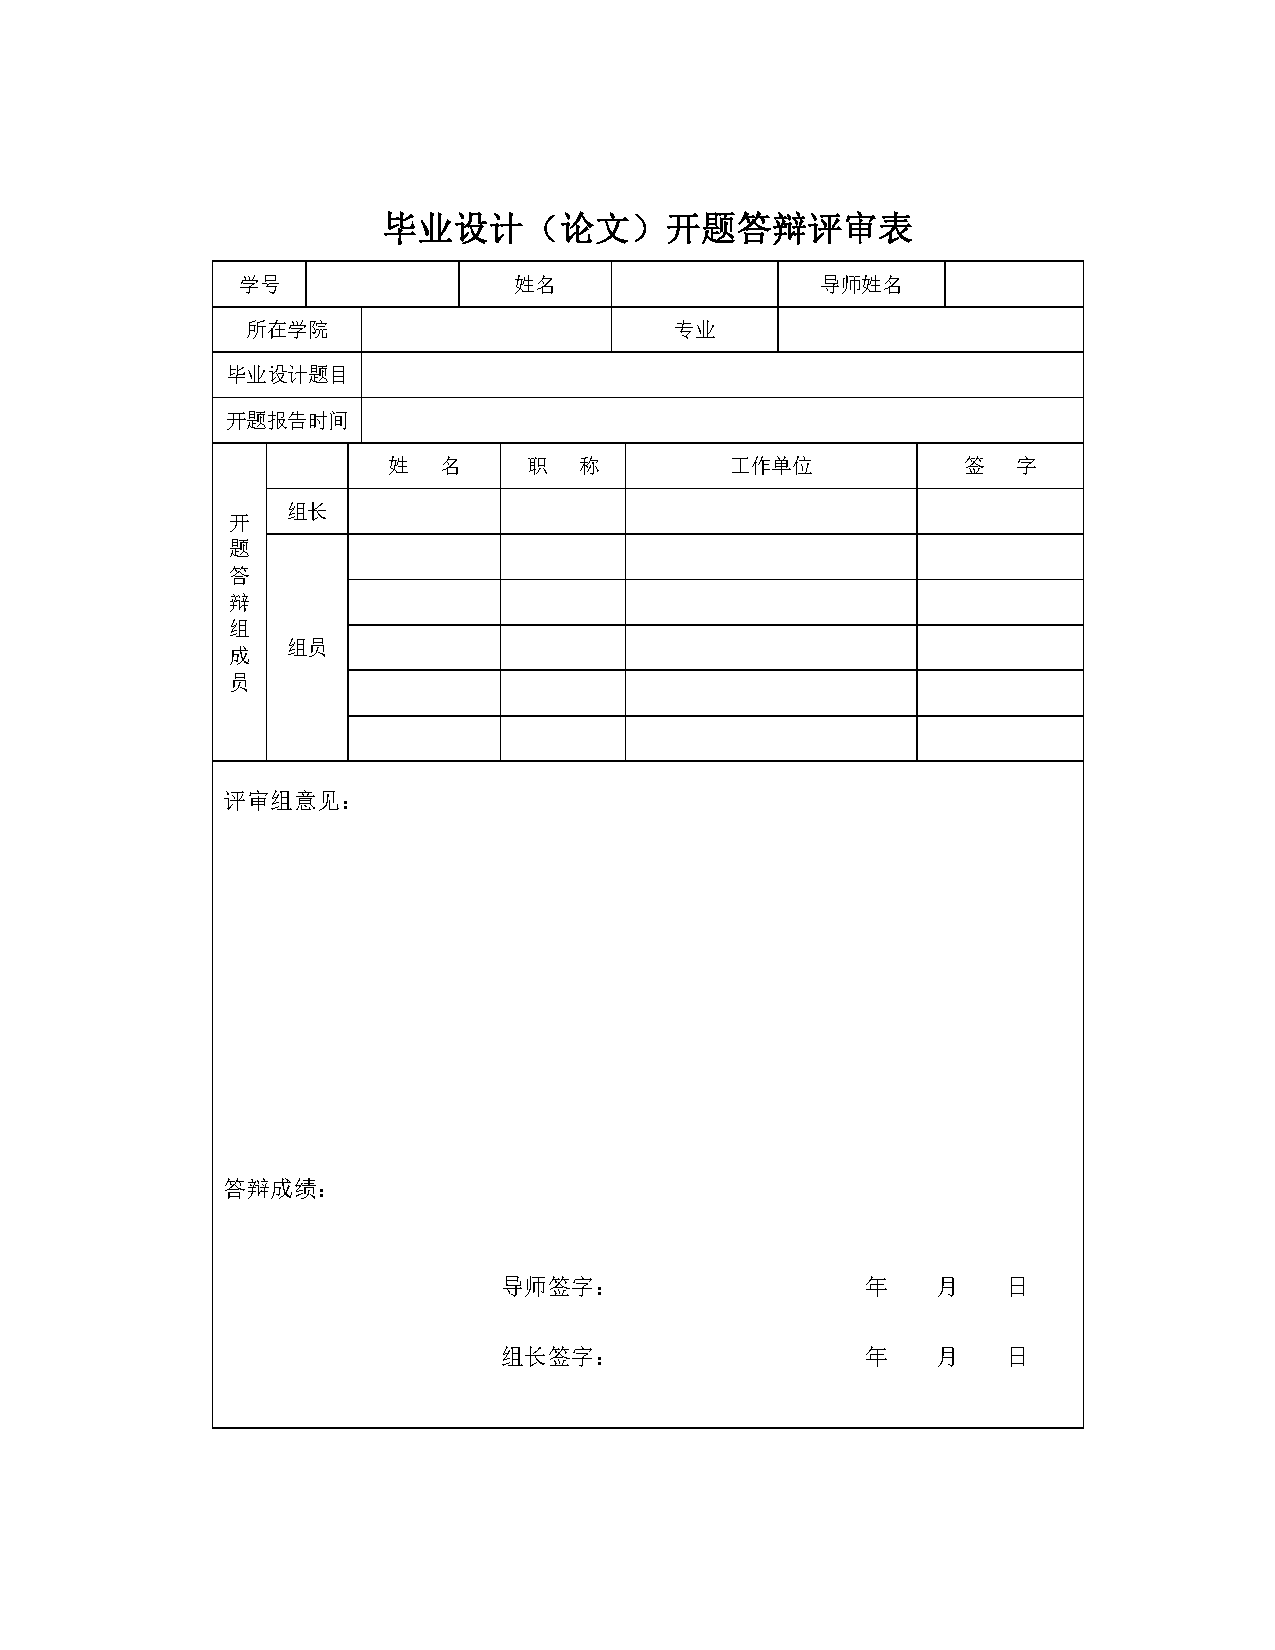
\includepdf[pages=-,scale=1.1]{misc/reviewTableBlank.pdf}

% 自动化学院开题报告中那些巨丑的框
\newtcolorbox{ubox}
{
	breakable,height fixed for=all,height fill,colback=white,arc=0mm,outer arc=0pt,width=1.01\linewidth,boxrule=.7pt,
	before upper={\parindent24bp},left=1.2pt,right=1.2pt,top=0mm,
}


%%
% 正文开始
\pagestyle{fancy}
% 正文从第一页开始计算页码
\setcounter{page}{1}
% 页眉和页脚(页码)的格式设定
\fancyhf{}

%\fancyhead[R]{\fontsize{10.5pt}{10.5pt}\selectfont{北京理工大学本科生毕业设计(论文)开题报告}}
\fancyfoot[C]{\fontsize{9pt}{9pt}\selectfont{\thepage}}
% 去掉header & footer的线
\renewcommand{\headrulewidth}{0pt}
\renewcommand{\footrulewidth}{0pt}

% 正文 22 磅的行距,段前段后间距为 0
\setlength{\parskip}{0em}
\renewcommand{\baselinestretch}{1.53}
% 正文首行悬挂 1.02cm
\setlength{\parindent}{1.02cm}

% 内容开始
\section{毕业设计(论文)任务书}
\begin{ubox}

\subsection{为什么用\LaTeX{}?}

至于为什么用\LaTeX{},其实很简单,因为用过都说香。具体香在哪呢,笔者就大致列举一下科研写作中最关心的一些问题$\text{\LaTeX}$是如何胜任的:
\begin{enumerate}
	\item 易于插入、管理文献
	\item 有了固定排版规则后只需要关注内容即可
	\item 插入图标公式方便,同时文章内的cross reference极其简单
\end{enumerate}

\subsection{题目内容}
开题报告总长度约 5 至 6 页,本部分重点介绍毕业设计选题的主要内容 \cite{LeCun2010},宋体,小三,段落前后 0.5 行。

\textbf{北京理工大学}(Beijing Institute of Technology)是中国共产党创办的第一所理工科大学,隶属于中华人民共和国工业和信息化部,副部级建制,是全国重点大学,首批进入世界一流大学建设高校A类行列,首批进入国家“211工程”、“985工程”,入选高等学校学科创新引智计划、高等学校创新能力提升计划、卓越工程师教育培养计划、国家建设高水平大学公派研究生项目、国家大学生创新性实验计划、国家级大学生创新创业训练计划、新工科研究与实践项目、中国政府奖学金来华留学生接收院校、首批高等学校科技成果转化和技术转移基地,是工业和信息化部高校联盟、中国人工智能教育联席会成员。

北京理工大学前身是1940年成立于延安的自然科学院,历经晋察冀边区工业专门学校、华北大学工学院等办学时期,1949年定址北京并接收中法大学校本部和数理化三个系,1952年定名为北京工业学院,1988年更名为\emph{北京理工大学}。


\subsection{任务要求}

\subsection{插入图片}
使用图片的方法如下,插入图片如下,\textbf{注意因为自动化学院要求开题报告必须有边框}(话说这个框真的没啥必要,更浪费纸了,而且还破坏了书写排版体验... )而这里的边框我使用的是\texttt{tcolorbox}环境,因此所有框内的float环境需要使用H选项。
\begin{figure}[H]
	\centering
	\includegraphics[width=0.4\linewidth]{example-image}
	\caption{一个图片例子}
	\label{fig:main}
\end{figure}

\subsection{引用图片的方法}
如图~\ref{fig:main}~所示... \textbf{注意}:由于是H环境因此需要注意图片的大小和放置位置,否则可能会产生不太好的效果(比如tcolorbox提前终止等)。

如果一个图由两个或两个以上分图组成时,各分图分别以(a)、(b)、(c)...... 作为图序,并须有分图题。
推荐使用 \texttt{subcaption} 宏包来处理, 比如图~\ref{fig:subfig-a} 和图~\ref{fig:subfig-b}。

\begin{figure}[H]
	\centering
	\subcaptionbox{分图 A\label{fig:subfig-a}}
	{\includegraphics[width=0.45\linewidth]{example-image-a.pdf}}
	\subcaptionbox{分图 B\label{fig:subfig-b}}
	{\includegraphics[width=0.45\linewidth]{example-image-b.pdf}}
	\caption{多个分图的示例}
	\label{fig:multi-image}
\end{figure}

\subsection{插入表格}

插入表格的方式如下,引用方式:如表~\ref{tab:demo}~所示...

\begin{table}[H]
	\centering
	\caption{示例表格}
	\label{tab:demo}
	\begin{tabular}[t]{lcc}
		\toprule
		&属性1&属性2\\
		\midrule
		张三&1&2\\
		李四&--&3\\
		王五&4&5\\
		\bottomrule
	\end{tabular}
\end{table}%
再举个例子,见表~\ref{tab:1}。
\begin{table}[H]
	\centering
	\caption{网络节点与边数统计}
	\begin{tabular}{ccc}
		\toprule
		\toprule
		年份    & 节点(上市公司)数   & 边数 \\
		\midrule
		2005  & 978   & 5,736 \\
		2006  & 1,002 & 5,691 \\
		2007  & 1,081 & 6,014 \\
		2008  & 1,141 & 6,132 \\
		\bottomrule
		\bottomrule
	\end{tabular}%
	\label{tab:1}%
\end{table}%
\end{ubox}


\newpage
\section{选题的背景和意义}
\begin{ubox}
\subsection{研究背景与意义}
本部分重点关注毕业设计的主要任务,宋体,四号,段落前后 0.5 行。

\subsection{国内外研究现状和发展趋势}
此部分要分析任务书,并给出初步方案,要体现出复杂系统的概念,约写 2 至 3 页。
\end{ubox}



\newpage
\section{研究方案}
\begin{ubox}
\subsection{数学公式与引用}

我想展示一下我的数学公式,比如下面这两个
\begin{equation}\label{eqn:demo}
	F = ma
\end{equation}
\begin{equation}
	N=m \frac{d^{2}}{d t^{2}}(x+l \sin \theta)
\end{equation}
引用的时候可以直接像这样,如公式~\ref{eqn:demo}~中所示...


\subsection{二级标题}

二级标题四号

\subsubsection{三级标题}

三级标题小四

\end{ubox}

\newpage
\section{实施技术方案所需要的条件}
\begin{ubox}
\subsection{参考文献}

参考文献使用\texttt{biber}进行编译,所有的\texttt{BibTeX}文件存于\texttt{ref.bib}内。
\subsection{}
\end{ubox}

\newpage
\section{预期成果}
\begin{ubox}
	内容...
\end{ubox}

\newpage
\section{时间安排}
\begin{ubox}
大致的课题计划进度如下表 \ref{tab:progress} 所示。

% 调整时间表的arraystretch
\renewcommand*\arraystretch{1.5} 
\begin{table}[H]
  \centering
  \caption{毕业设计计划进度表}
  \label{tab:progress}
  \begin{tabular}{@{}cc@{}}
    \toprule
    时间 & 计划完成工作       \\ \midrule
    3.1—3.8 & 撰写开题报告,完成开题答辩 \\\hline
    & \\\hline
    & \\\hline
    6.3—6.11 & 完成最终答辩\\\bottomrule
  \end{tabular}

\end{table}

\end{ubox}

\newpage
\section{参考文献}
\begin{ubox}
% 删除默认的「参考文献 / Reference」标题,使用上面定义的 section 标题
\CJKunderline{注意}:下文的参考文献应包含近 5 年内文献,经典文献除外。 参考文献已使用规定的\texttt{GB/T 7714-2015}标准(使用时请删掉这句话)
\printbibliography[heading=none]
\end{ubox}


\end{document}
